\documentclass{beamer}

\usefonttheme{professionalfonts} % using non standard fonts for beamer
\usefonttheme{serif} % default family is serif

\usepackage{hyperref}
%\usepackage{minted}
\usepackage{animate}
\usepackage{graphicx}
\def\Put(#1,#2)#3{\leavevmode\makebox(0,0){\put(#1,#2){#3}}}
\usepackage{colortbl}
\usepackage{tikz}
\usepackage{amssymb}
\usepackage{enumerate}
\usepackage{arydshln}
\usepackage{algorithm}
\usepackage{algpseudocode}

\colorlet{lightred}{red!25}
\colorlet{lightgreen}{green!25}


\newcommand\blfootnote[1]{%

  \begingroup

  \renewcommand\thefootnote{}\footnote{#1}%

  \addtocounter{footnote}{-1}%

  \endgroup

}

\makeatletter

%%%%%%%%%%%%%%%%%%%%%%%%%%%%%% Textclass specific LaTeX commands.

 % this default might be overridden by plain title style

 \newcommand\makebeamertitle{\frame{\maketitle}}%

 % (ERT) argument for the TOC

 \AtBeginDocument{%

   \let\origtableofcontents=\tableofcontents

   \def\tableofcontents{\@ifnextchar[{\origtableofcontents}{\gobbletableofcontents}}

   \def\gobbletableofcontents#1{\origtableofcontents}

 }

%%%%%%%%%%%%%%%%%%%%%%%%%%%%%% User specified LaTeX commands.

\usetheme{Malmoe}

% or ...

\useoutertheme{infolines}

\addtobeamertemplate{headline}{}{\vskip2pt}

\setbeamercovered{transparent}

% or whatever (possibly just delete it)

\makeatother

\begin{document}
\title[PFLOCK report]{PFLOCK Report}
\author[AC]{Andres Calderon}
\institute[Winter'20]{University of California, Riverside}
\makebeamertitle
\newif\iflattersubsect

\AtBeginSection[] {
    \begin{frame}<beamer>
    \frametitle{Outline} 
    \tableofcontents[currentsection]  
    \end{frame}
    \lattersubsectfalse
}

\AtBeginSubsection[] {
    \begin{frame}<beamer>
    \frametitle{Outline} 
    \tableofcontents[currentsubsection]  
    \end{frame}
}

\begin{frame}{The problems...}
    \begin{itemize}
        \item A few very large tasks.
        \item Unbalance distributions of tasks.
    \end{itemize}

    \begin{figure}
        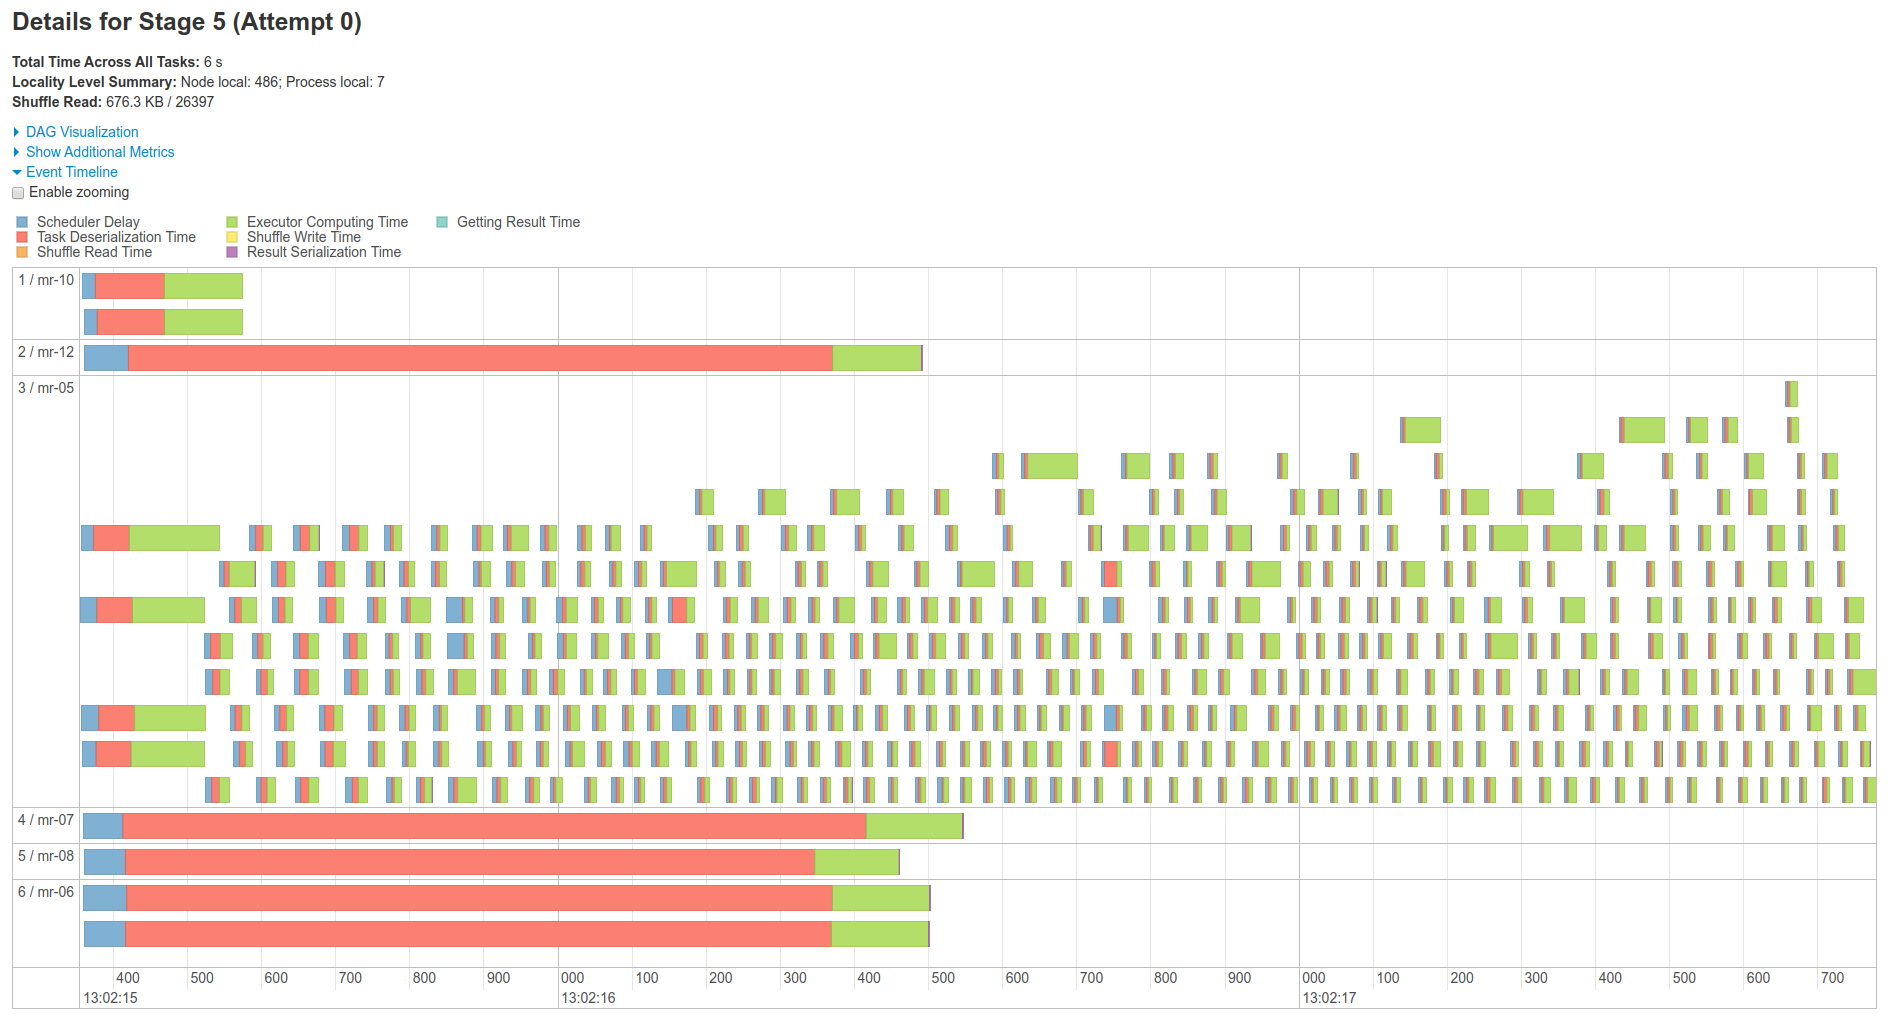
\includegraphics[width=0.9\textwidth]{figures/Problem}
    \end{figure}
\end{frame}

\begin{frame}{Solution 1...}
    \begin{itemize}
        \item Most of the time is for deserialization (time sending task closure to executor: i.e. code, libraries and data).
        \item It has to be done once per executor.
        \item Solution: force repartition at the very beggining to initialize all the executors.
    \end{itemize}
\end{frame}

\begin{frame}{Solution 2...}
    \begin{itemize}
        \item Spark does not distribute tasks correctly for RDD with less than 1000 partitions.
    \end{itemize}

    \begin{figure}
        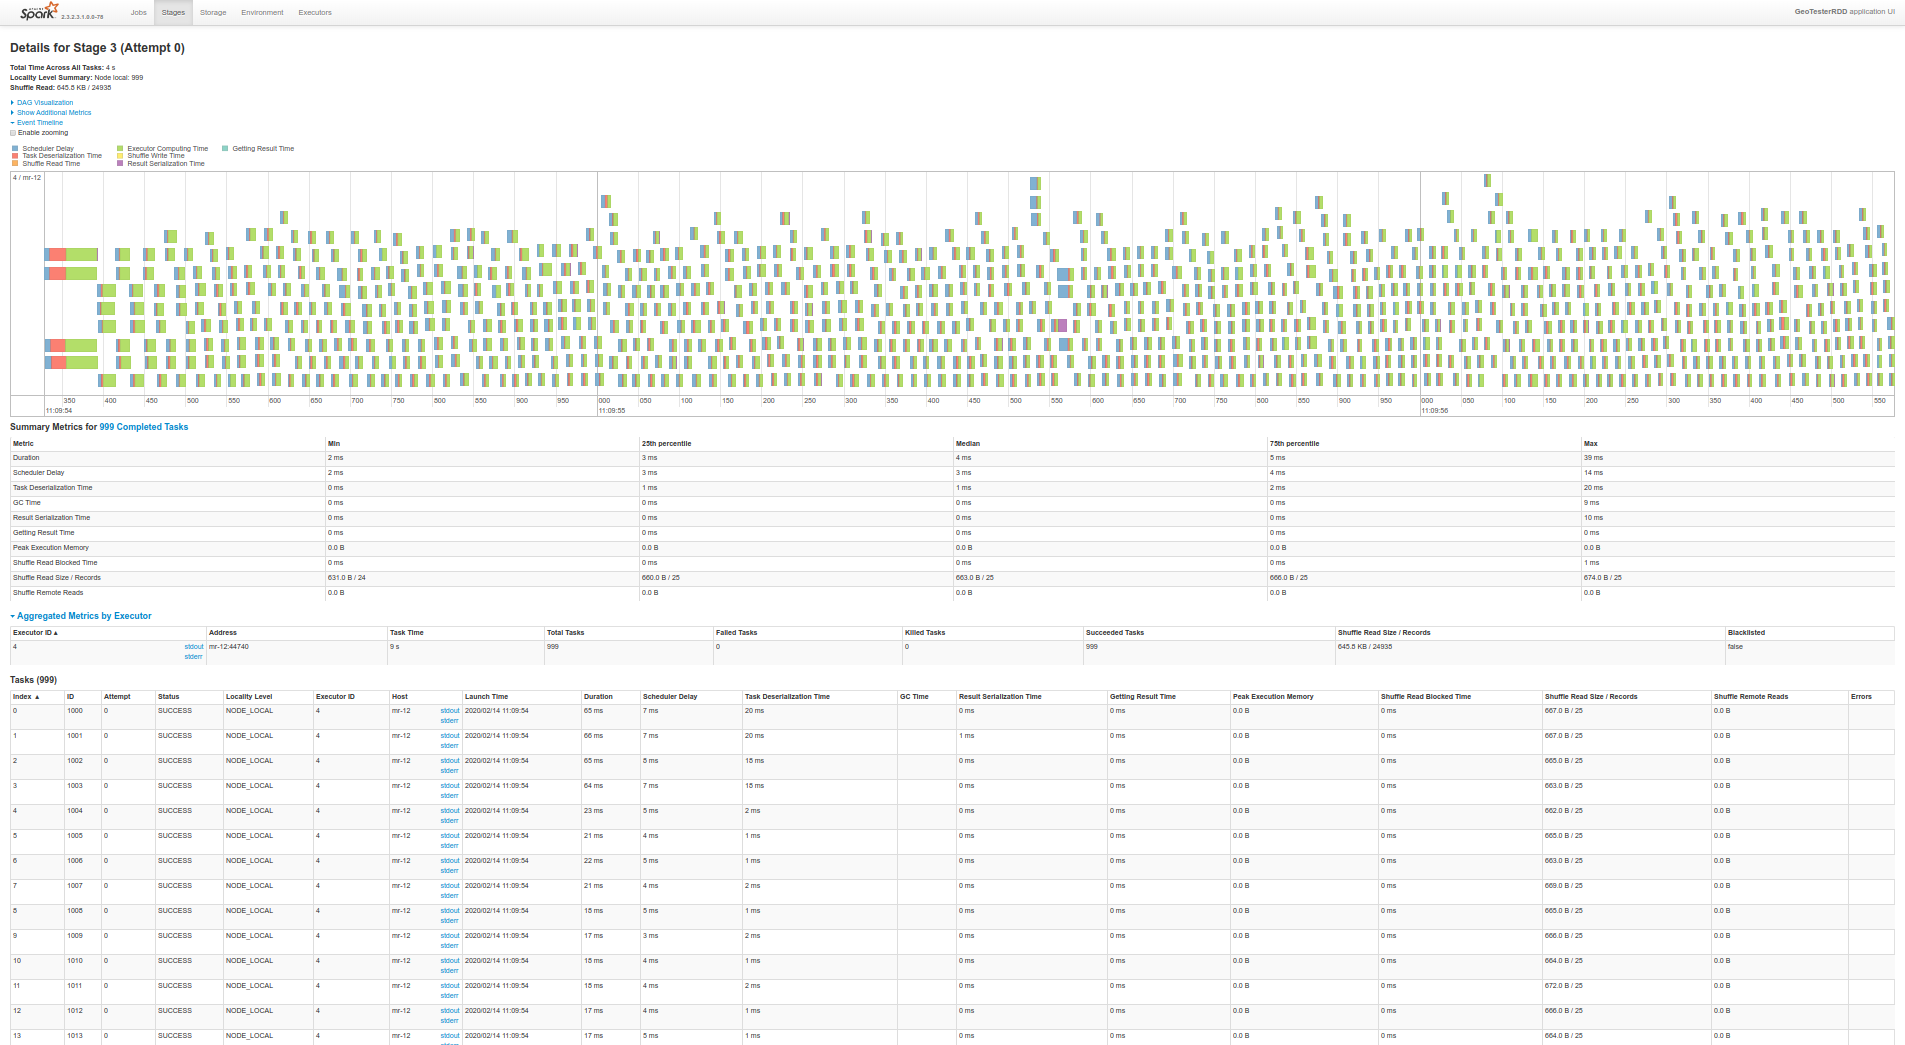
\includegraphics[width=0.8\textwidth]{figures/P999S3}
        \caption{999 partitons}
    \end{figure}
\end{frame}
\begin{frame}{Solution 2...}
    \begin{itemize}
        \item Spark does not distribute tasks correctly for RDD with less than 1000 partitions.
    \end{itemize}

    \begin{figure}
        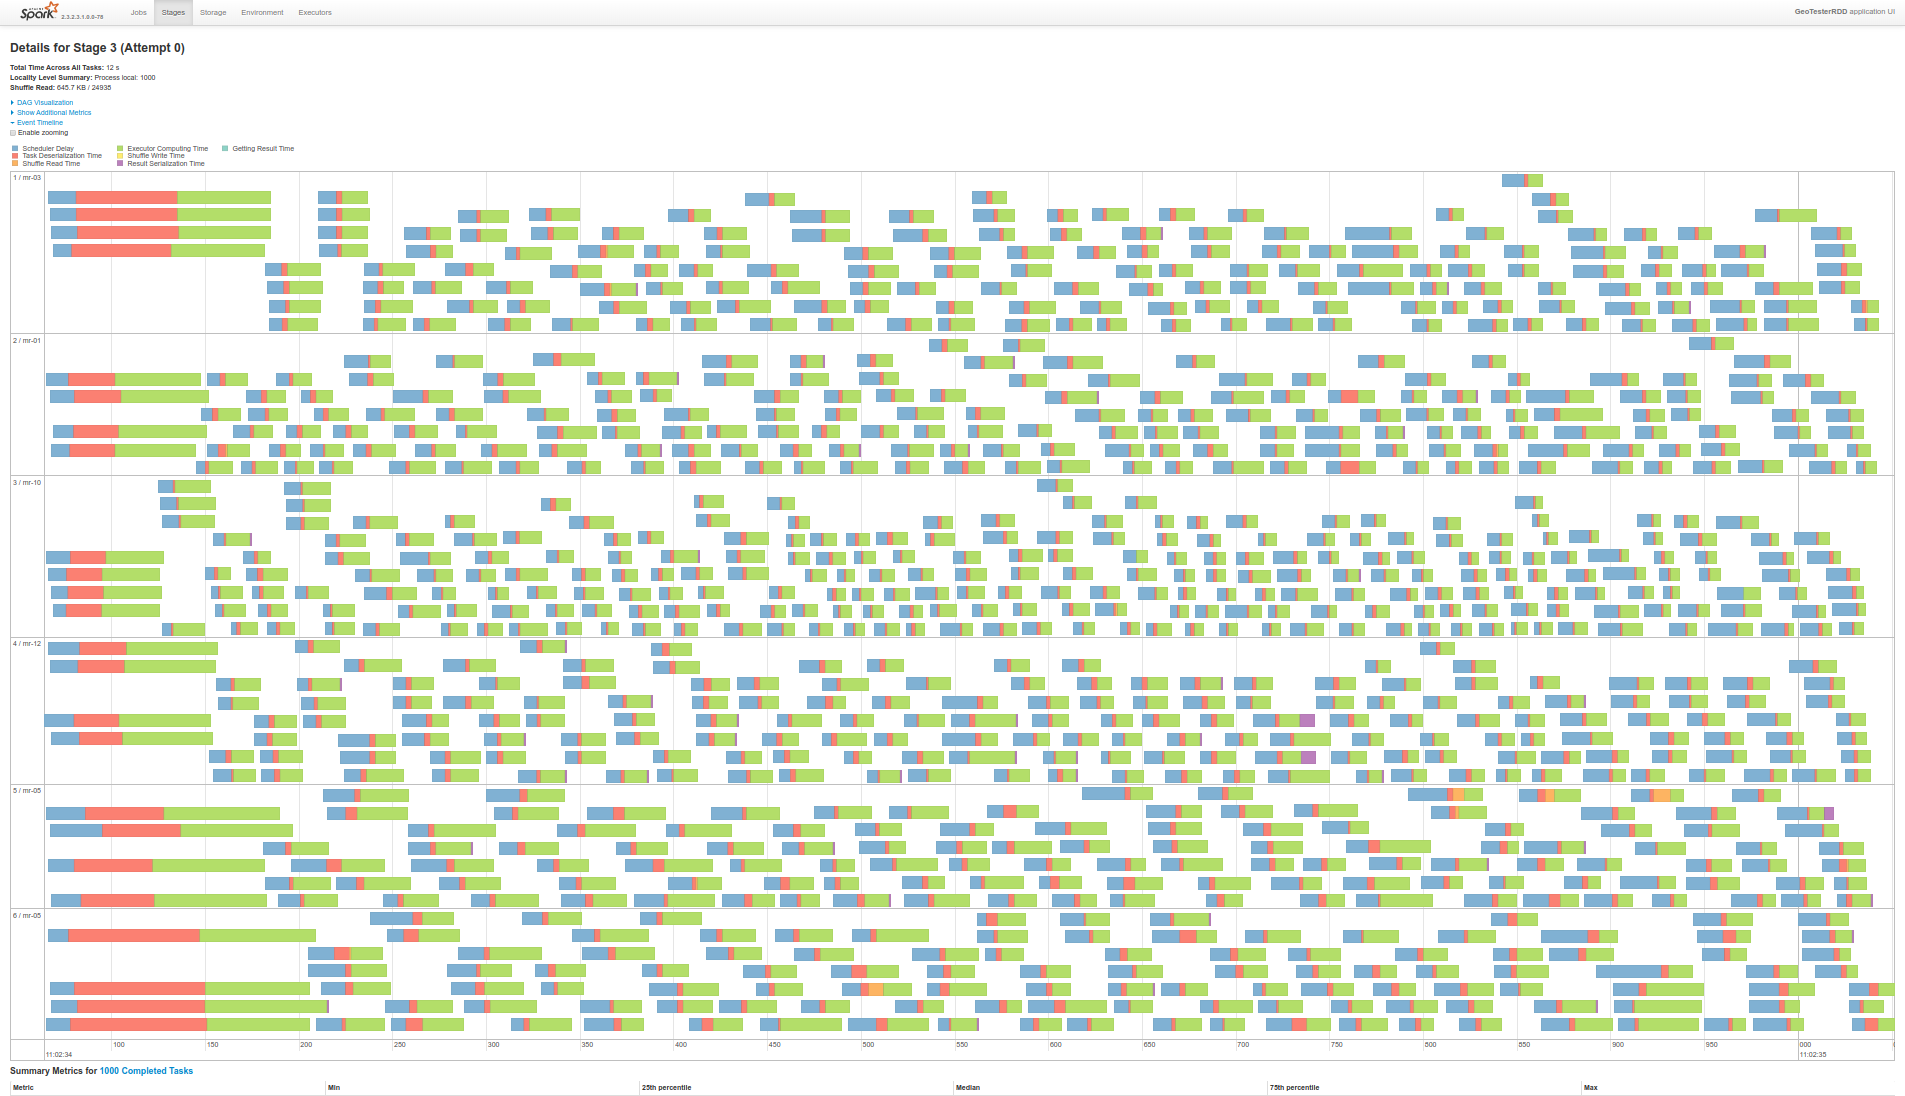
\includegraphics[width=0.8\textwidth]{figures/P1000S3}
        \caption{1000 partitons}
    \end{figure}
\end{frame}

\begin{frame}{General performance...}
    \begin{figure}
        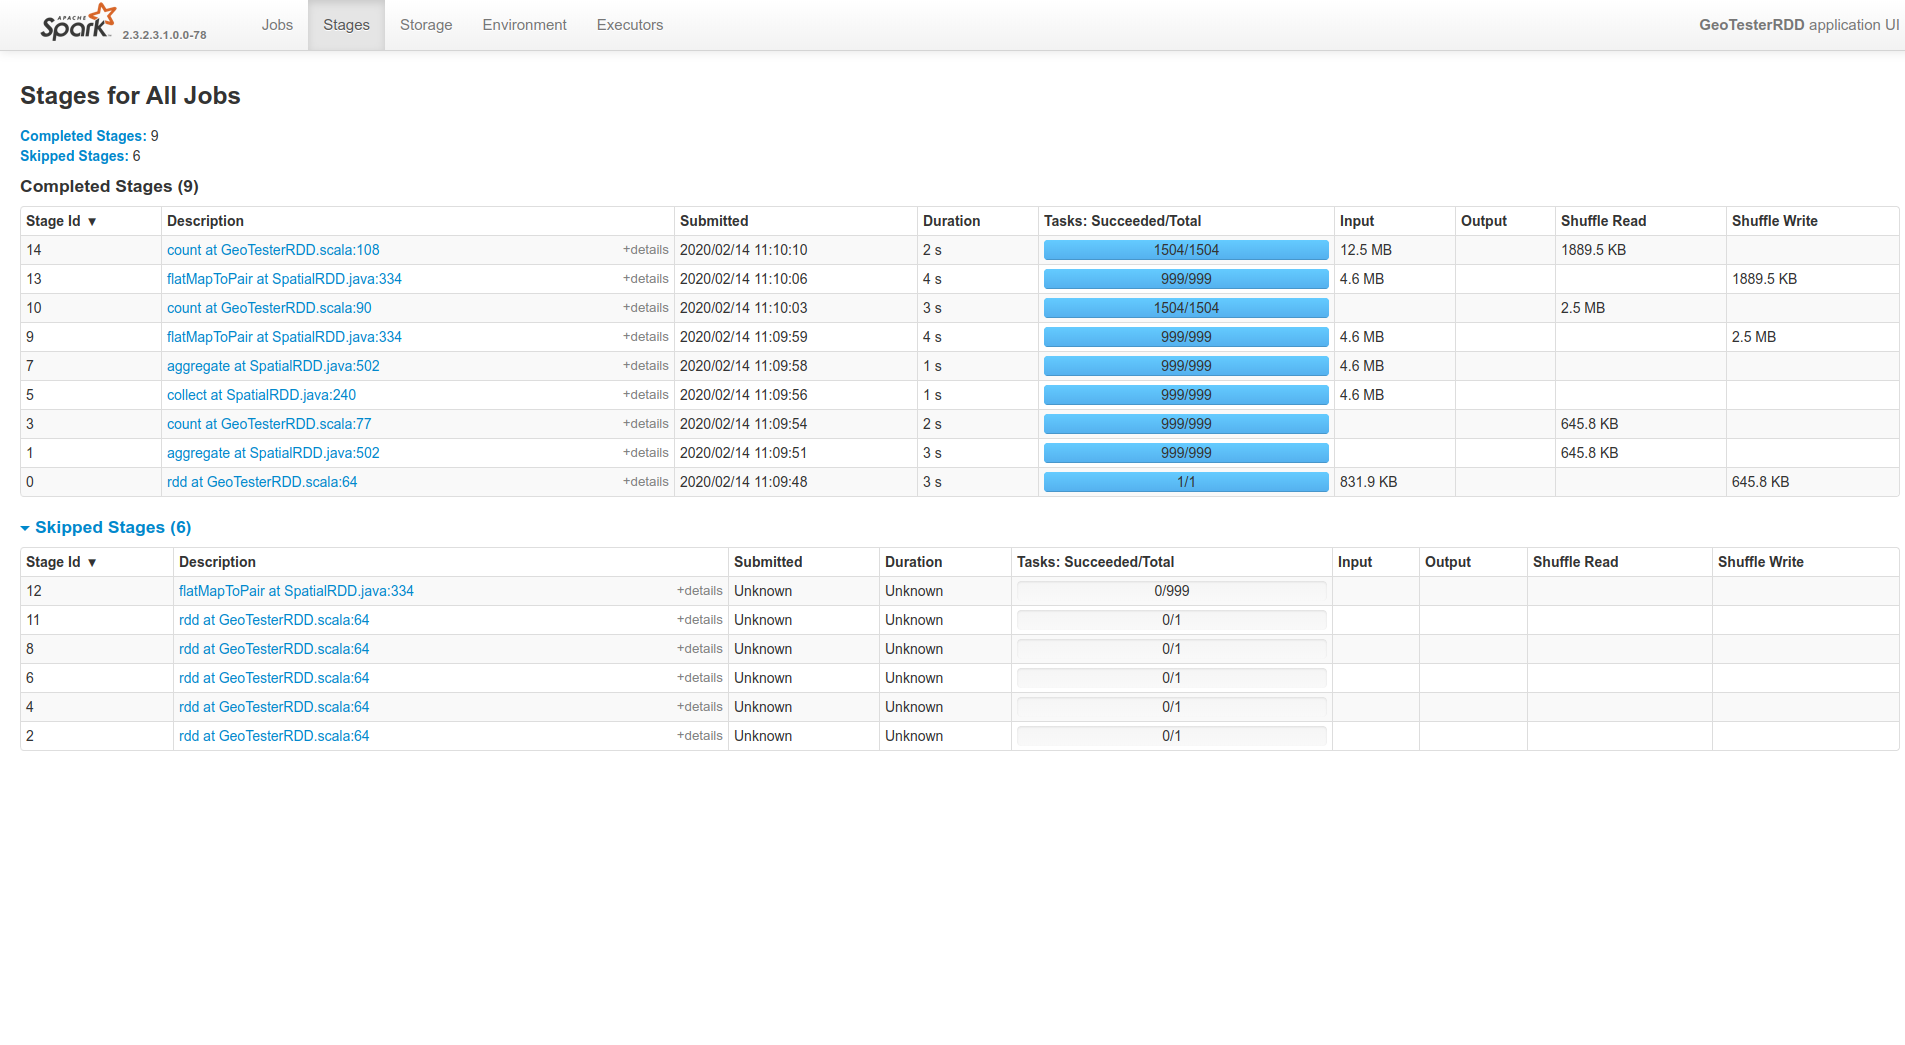
\includegraphics[width=\textwidth]{figures/P999}
        \caption{999 partitons}
    \end{figure}
\end{frame}
\begin{frame}{General performance...}
    \begin{figure}
        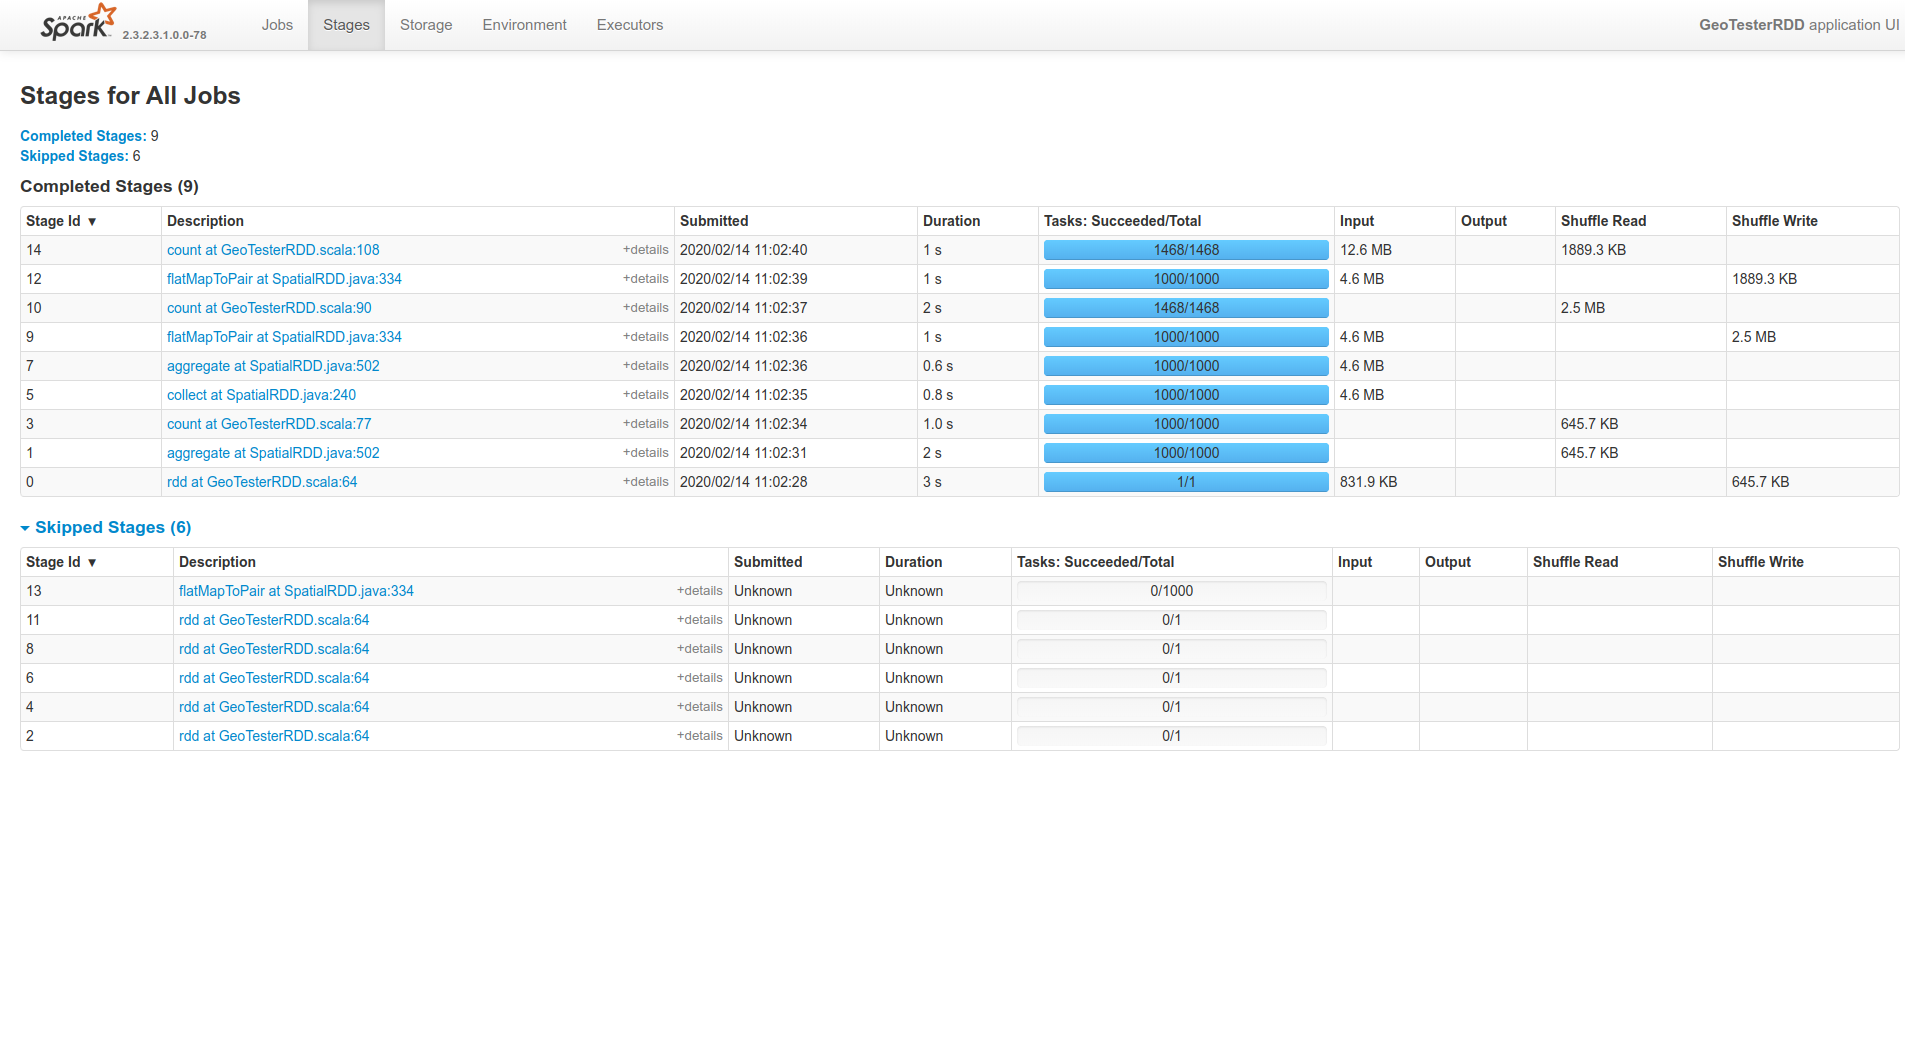
\includegraphics[width=\textwidth]{figures/P1000}
        \caption{1000 partitons}
    \end{figure}
\end{frame}

\begin{frame}{Distance self-join stage...}
    \begin{figure}
        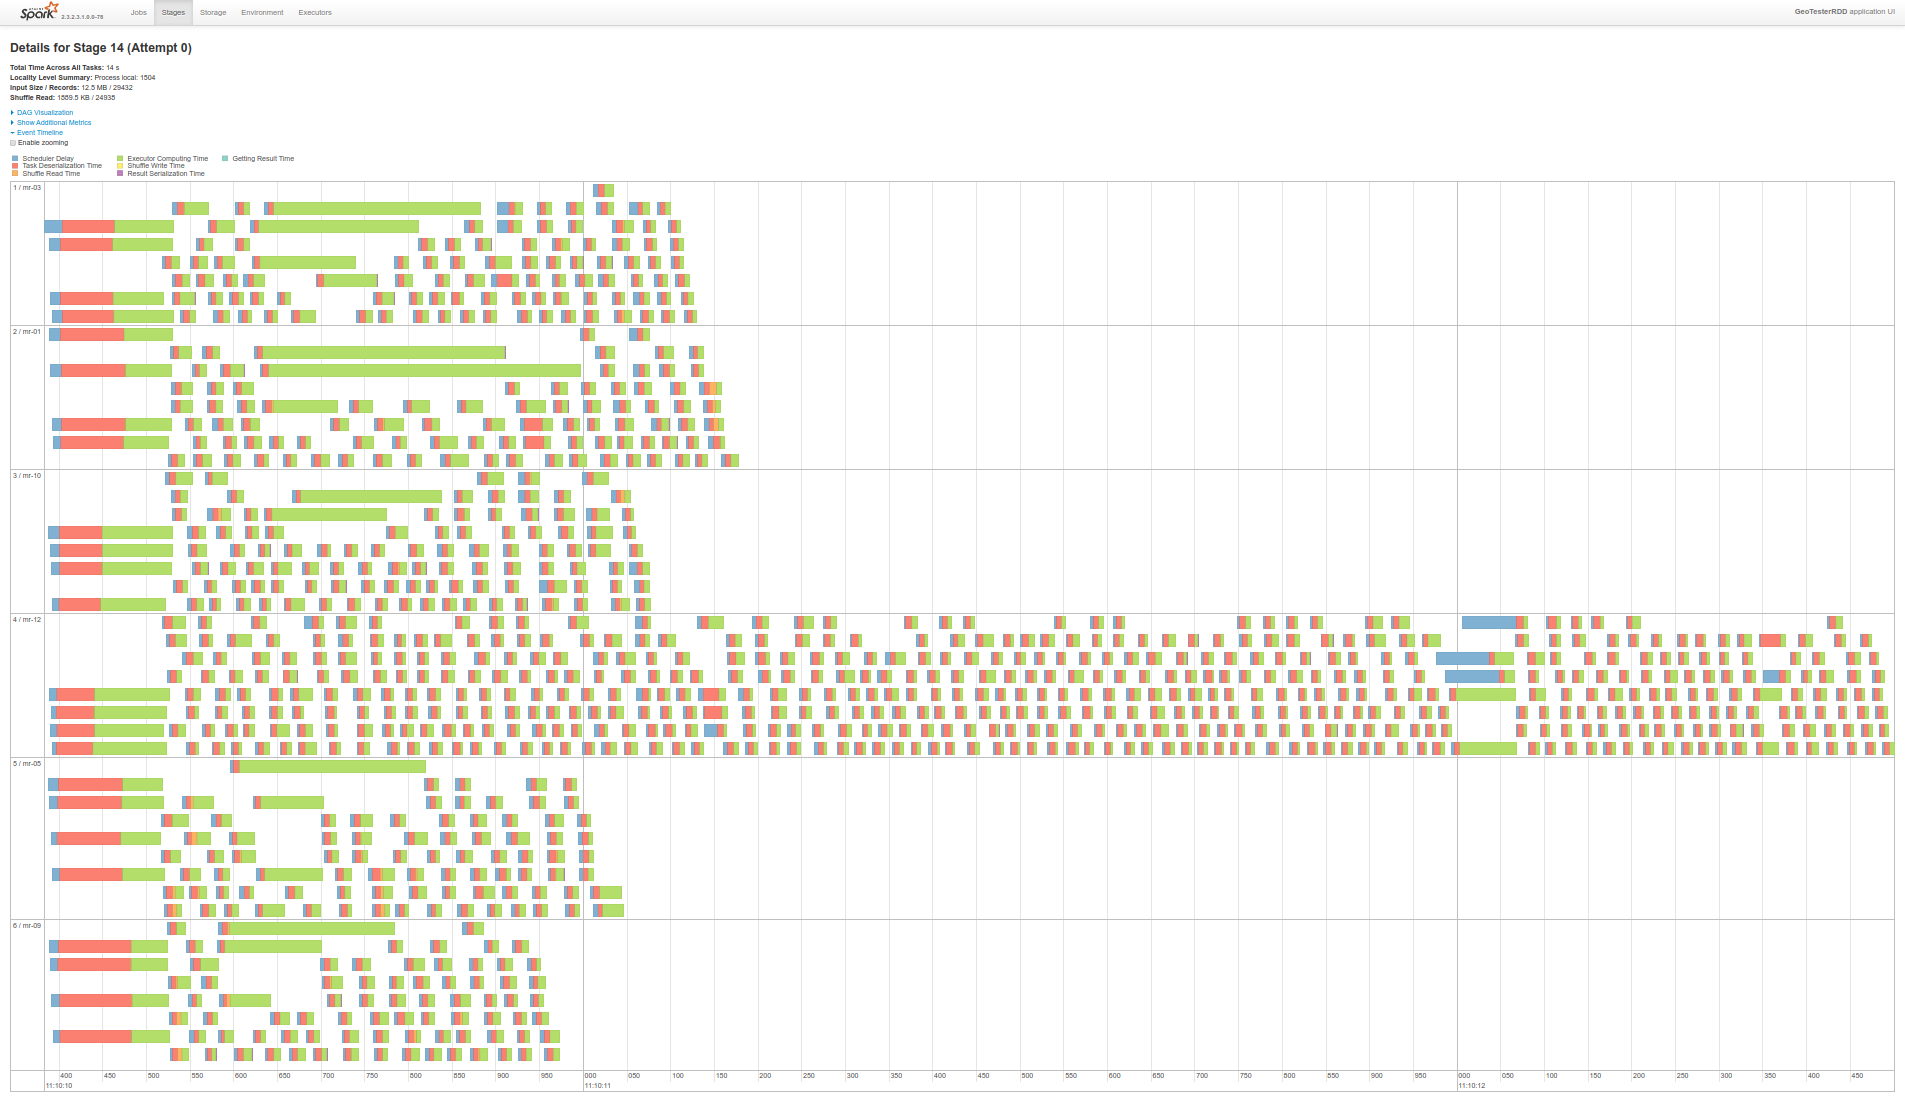
\includegraphics[width=\textwidth]{figures/P999S13}
        \caption{999 partitons}
    \end{figure}
\end{frame}
\begin{frame}{Distance self-join stage...}
    \begin{figure}
        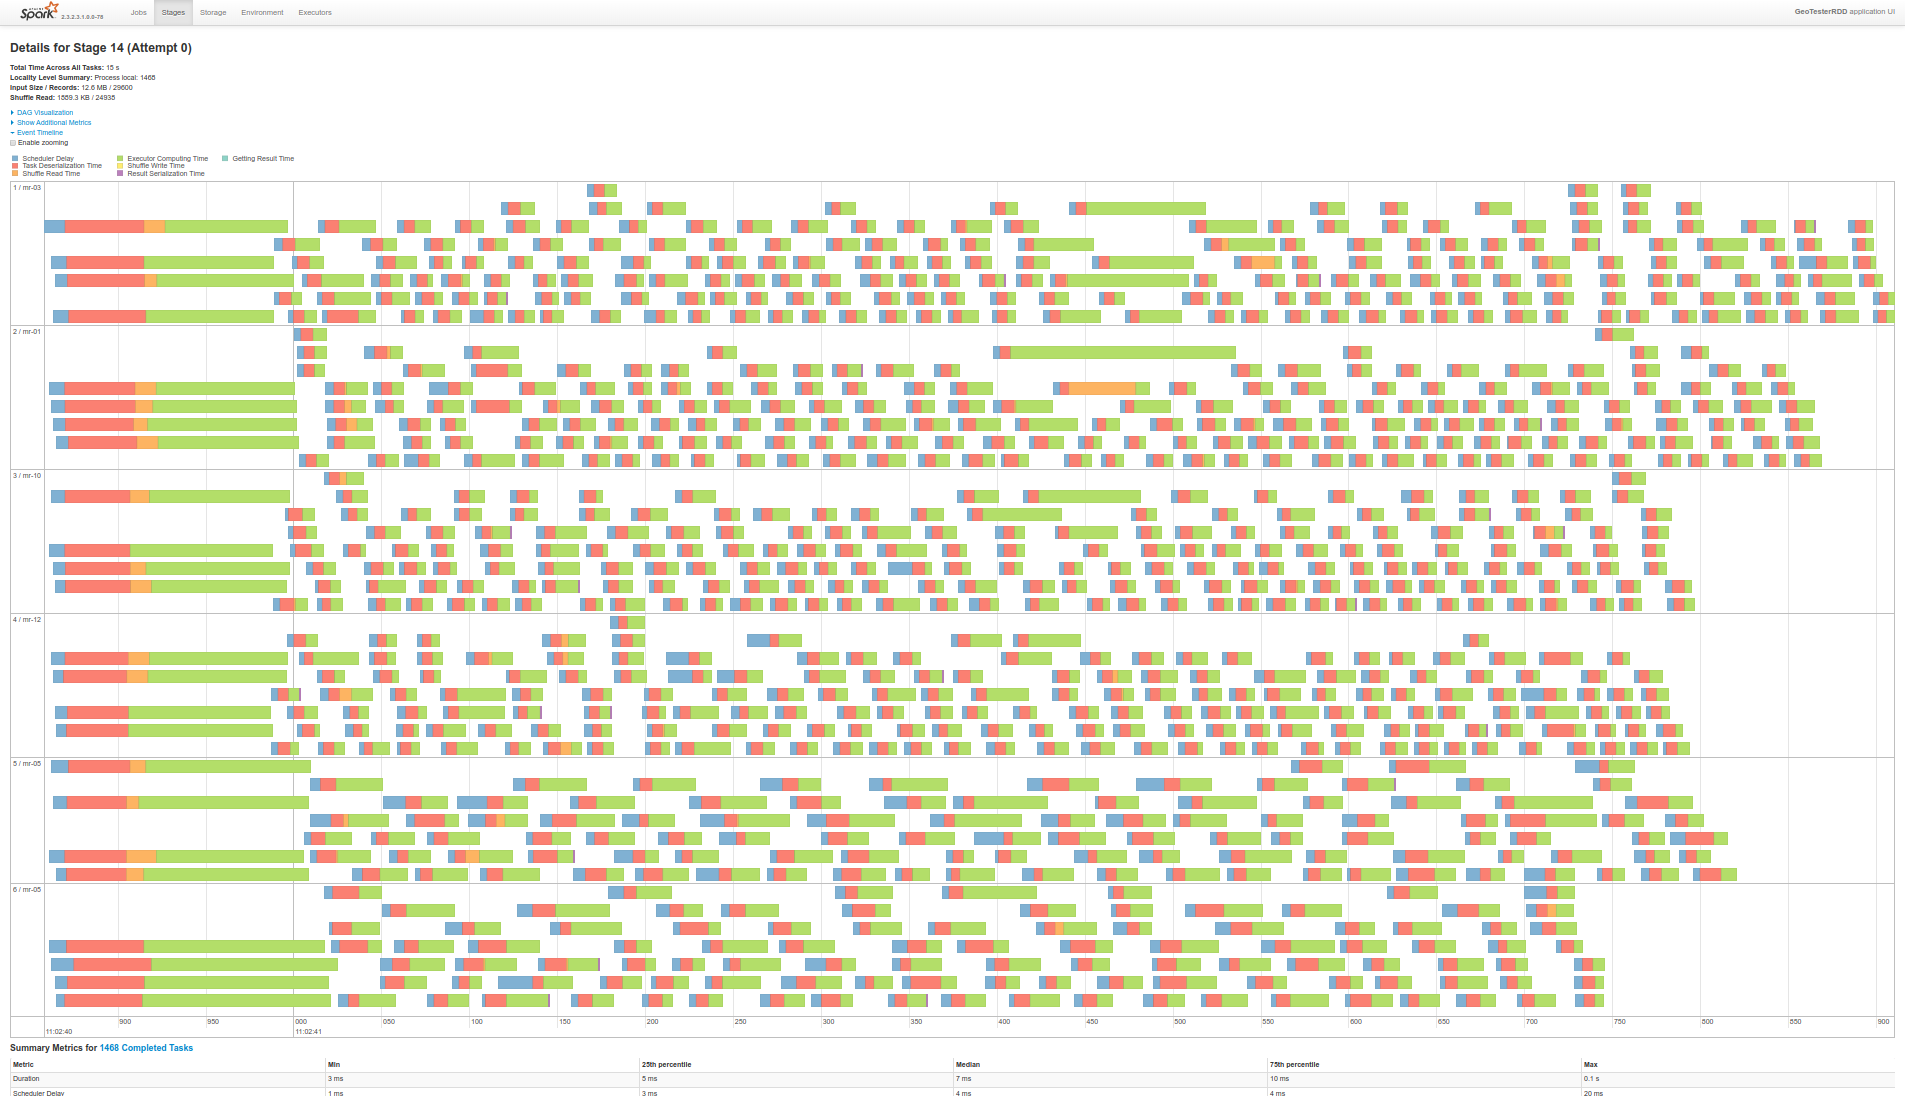
\includegraphics[width=\textwidth]{figures/P1000S13}
        \caption{1000 partitons}
    \end{figure}
\end{frame}
\begin{frame}{Distance self-join task summary...}
    \begin{figure}
        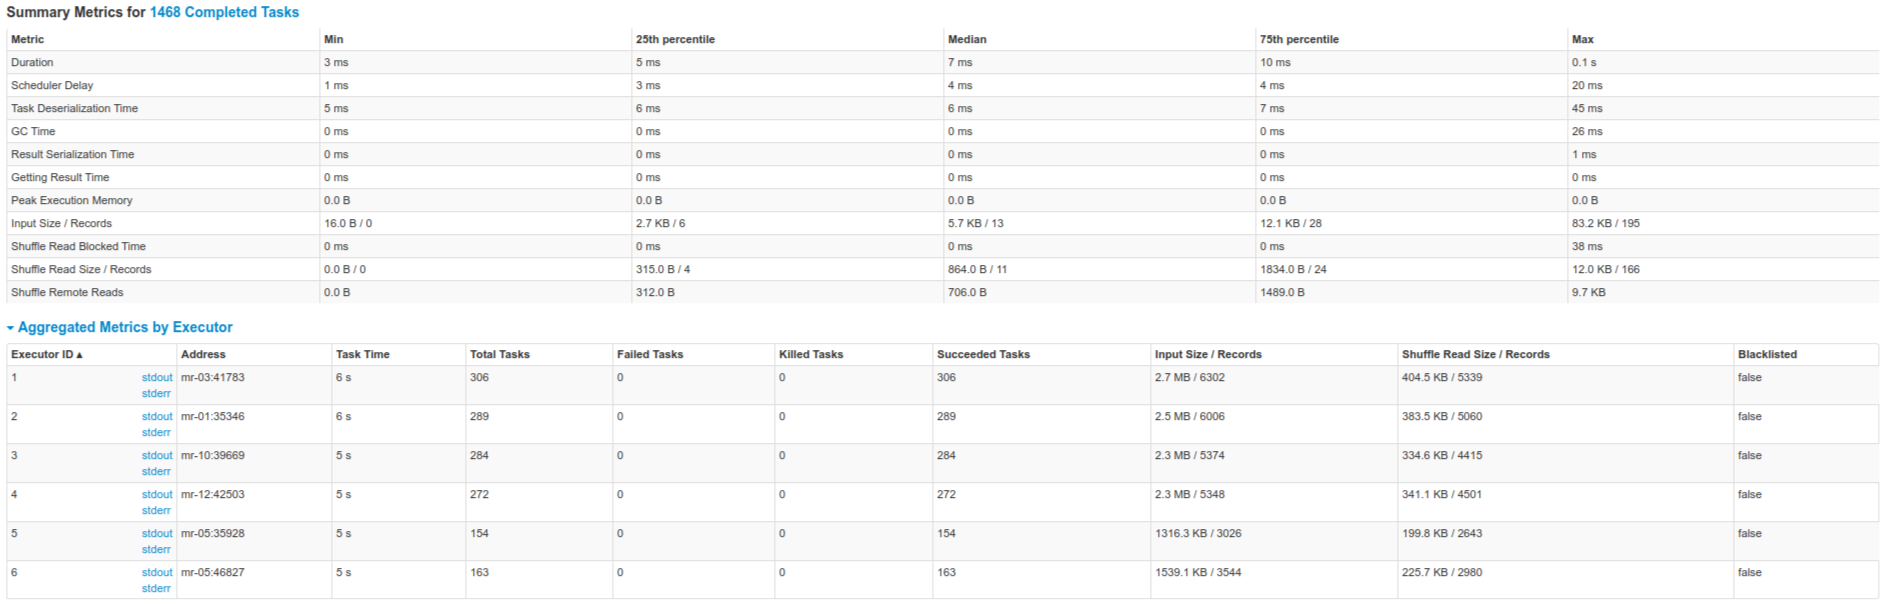
\includegraphics[width=\textwidth]{figures/Summary1000}
        \caption{1000 partitons}
    \end{figure}
\end{frame}
\begin{frame}{Distance self-join task details...}
    \begin{figure}
        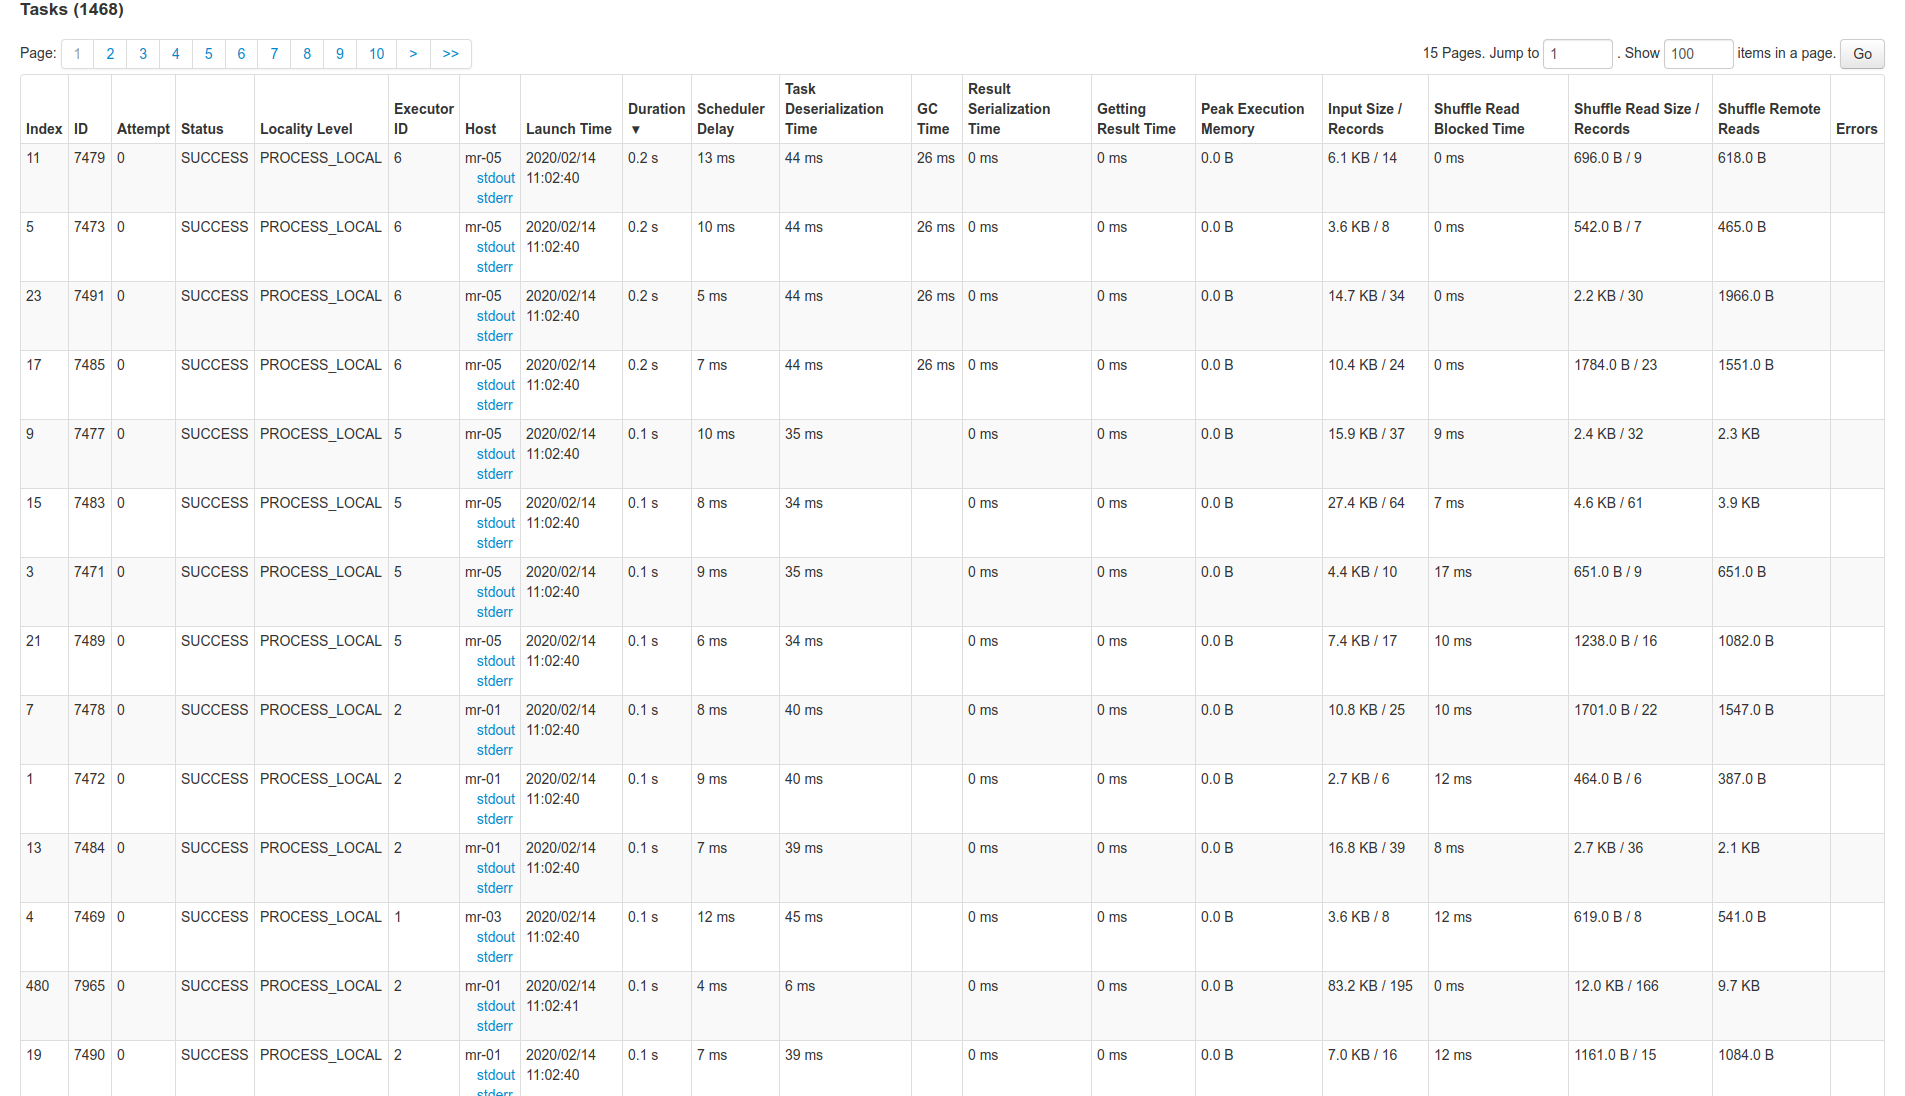
\includegraphics[width=\textwidth]{figures/Tasks1000}
        \caption{1000 partitons}
    \end{figure}
\end{frame}
\end{document}
